\chapter{Results}
\label{ch:results}

\section{Overview}

This chapter outlines the outcomes of the individual BLISS system blocks and evaluates their performance and realiseability.  Since a large transistion was made from original research and goals, many limitations were enforced in the final design presented in this thesis.  Feasibility was desired during the implementation stage of this work, causing this transition, but full implementations were produced in the end.  Since certain channel conditions couldn't be replicated in reality baseline evaluations were produced for proof of concept, and rigorious hardening is a viable path for future work.\\ 

\section{Spectral Subtraction}

The goal of this section is to present the results of the Spectral Subtraction signal processing block.  This block, as mentioned in previous sections, tries to remove non-orthoganol signals from the spectrum that are located on the same frequency of the desired signal.  This mimics the effects of a wideband jamming system, causing all effective bandwidth or throughput to diminish.  

In order to operate this system assumes

\subsection{Experiment}

This experiment consists of four USRP2 radio transceivers.  One radio acting as a transmitter, one the interferer, and two receive radio connected through a MIMO-USRP cable.  The cable causes direct synchronization between the receive radios.  This is required to perform maximal ratio combining to correctly align signals constructively.  During the test the interferer first begins transmitting data, then the desired transmitter begins to transmit.  At all times the receiver is actively receiving all signals in the spectrum.  Since noise energy could not be adjusted baseline feasibility was demonstrated.\\

All transmissions utilize GMSK, due to its resilience to changes in the radio's power amplifier.  All radios operate at 100kbits/sec, well under the maximum rate of the radios, minimizing the load on the machines themselves and the amount of data generated.  The machines connected to the radios are all Core Series Intel processing, installed with Ubuntu Linux 10.10 and 12.04.  All machines were also running MATLAB 2011B, and GNU-Radio 3.6.2git-145-g7c8347ca built from the git repository.  All signal recordings/reception was done in GNU-Radio and all signal processing at baseband was done in MATLAB.\\  

Here is a picture of the experimental setup with all four radios:

\being{figure}\label{ss_setup_real}
\includegraphics{ss_setup_real.eps}
\end

To evaluate the Spectral Subtraction block the signal was demodulated, timing recovered, and compared against the transmitted data.  Mueller Muller timing was used as a timing recovery method.  Several runs were made, and varying results were recorded.  Since the frequency drift of the USRP2 crystal oscillators, which control the transmission and reception frequencies, can vary on the order of kilohertz.  This non-ideality seemed to be the most difficult problem to compenstate for, since it couldn't be directly measured when the signals were mixed.  A visual inspection of the subtracted result show an oscillating error in the spectrum which is shown in figure \ref{ss_oscillation}.  As express previously, Spectral Subtraction is very susceptable to data corruption.  It is analogous to hitting a moving target, since the operation is extremely time varying and time dependent.\\  


\begin{figure}\label{ss_oscillation}
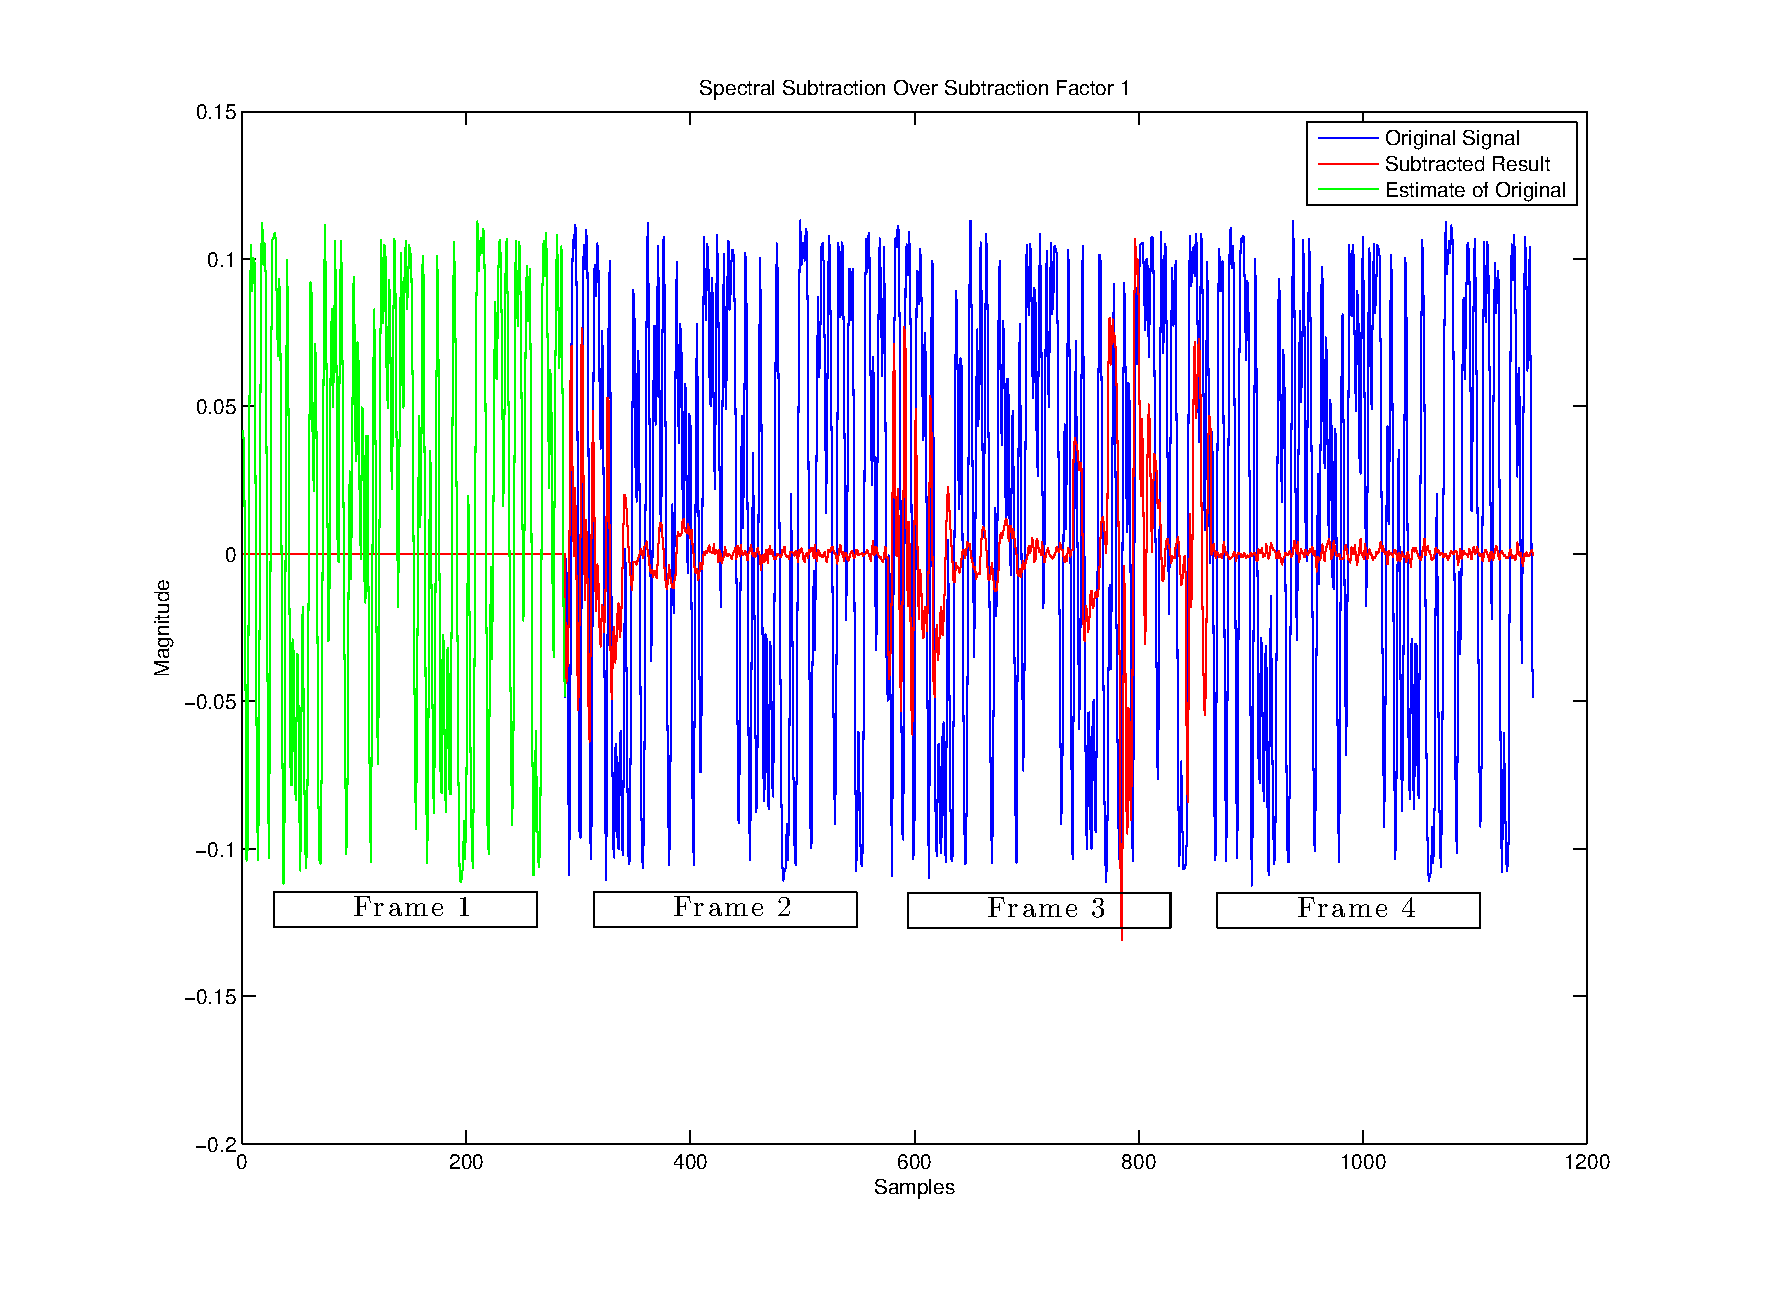
\includegraphics{ss_oscillation.eps}
\end

Since noise couldn't be varied in this implementation for direct comparision against simulation, presented is a series of runs and their coinciding errors.  Each run only represents the periods for which the signals are mixed, which is roughly 3 seconds.  The error represents the accuracy of the demodulated signal and not the amount of unwanted still existing in the channel, since it is less desired.  This data can be seen in figure \ref{ss_error_runs}.\\

%\begin{figure}\label{ss_error_runs}
%\includegraphics{ss_error_runs.eps}
%\end

\subsection{Analysis}

Spectral Subtraction in a extremely well studied area in signal processing, but no existing literature exists for its application in a digital communication system.  It has been shown here that it can be quite difficult for it to be applied, even under serious constraints.  Under the conditions of this thesis, the assumptions are quite reasonable, but due to the large amount of error in the results, more may need to be considered.  These may include accuracy requirements for physical equipment, primarily to reduce carrier frequency drift.  Burst scenarios may also be considered to reduce bit error rate.  Overall, for a completely non-existant field of study, these results point the possibility of operational success.  Future work will we required, especially during the implementation phase of designs.\\

\section{Signal Separation}

The Signal Separation block changed the most from the original research design.  Much of the design needed to be reconsidered because of time constraints and lack of robust research conclusions.  The design distilled down to a combination of Maximal Ratio Combining and adaptive equalization.  Two well know concepts in communication system design, and rather straight forward to implement.  Maximal Ratio Combining provides the benefits of maximizing the spectrum spacially, while also adaptively equalizing these separated data streams to help remove corruption left over by spectral subtraction of the channel itself.  The more dimensionality that can be exploited the more performance can be extracted.\\

\subsection{Experiment}

Signal Separation utilized an identical setup as the Spectral Subtraction testing, which is quite obvious since Signal Separation is downstream from Spectral subtraction in the data path.  To separate problems or issues with the performance of the Spectral Subtraction block it is removed from the data path, providing direct analysis and evaluation of the Signal Separation block.  It takes in two data stream, which have been timing synchronize through the use of the MIMO USRP cable.  These streams are equalized by an LMS Adaptive equalizer of length 14.  These taps provided the Maximal Ratio Combining weight analysis, providing information on which of the channel was less corrupted.  This is done by combining the filter tap values and taking the ratio of the two equalizers, and these weights determine how much of each signal is added to the final output signal.\\ 

Again all transmissions utilize GMSK, due to its resilience to changes in the radio's power amplifier.  All radios operate at 100kbits/sec, well under the maximum rate of the radios, minimizing the load on the machines themselves and the amount of data generated.  The machines connected to the radios are all Core Series Intel processing, installed with Ubuntu Linux 10.10 and 12.04.  All machines were also running MATLAB 2011B, and GNU-Radio 3.6.2git-145-g7c8347ca built from the git repository.  All signal recordings/reception was done in GNU-Radio and all signal processing at baseband was done in MATLAB.  Therefore the entire Signal Separation block resides in MATLAB.\\  

Several separate transmissions were made and baseline bit error rates were calculated.  This was done by quantizing the final output and comparing the results.  The Mueller Muller method again was used for timing recovery due to its robustness.  It doesn't account for bit slips, but due to the rather short periods of transmission these can be ignored.  Since this block is designed to help in rather noisy and localized corruption situations, it can be very hard to test because there is no control over the spectral environment to set such conditions.  Rather this design shows a proof of concept with just SDR technology.  The results for the baseband tests are shown in figure \ref{ssep_results}.\\

\begin{figure}\label{ssep_results}
\includegraphics{ssep_results.eps}
\end

\subsection{Analysis}

From the results seen from the baseline testing, reception seems to be quite flawless. To provide a comparision to the simulated results, the transmitter power was lowered to synthetically reduce the SNR of the signal.  The results of these tests can be seen in figure \ref{ssep_snr_tests}.   

\begin{figure}\label{ssep_snr_tests}
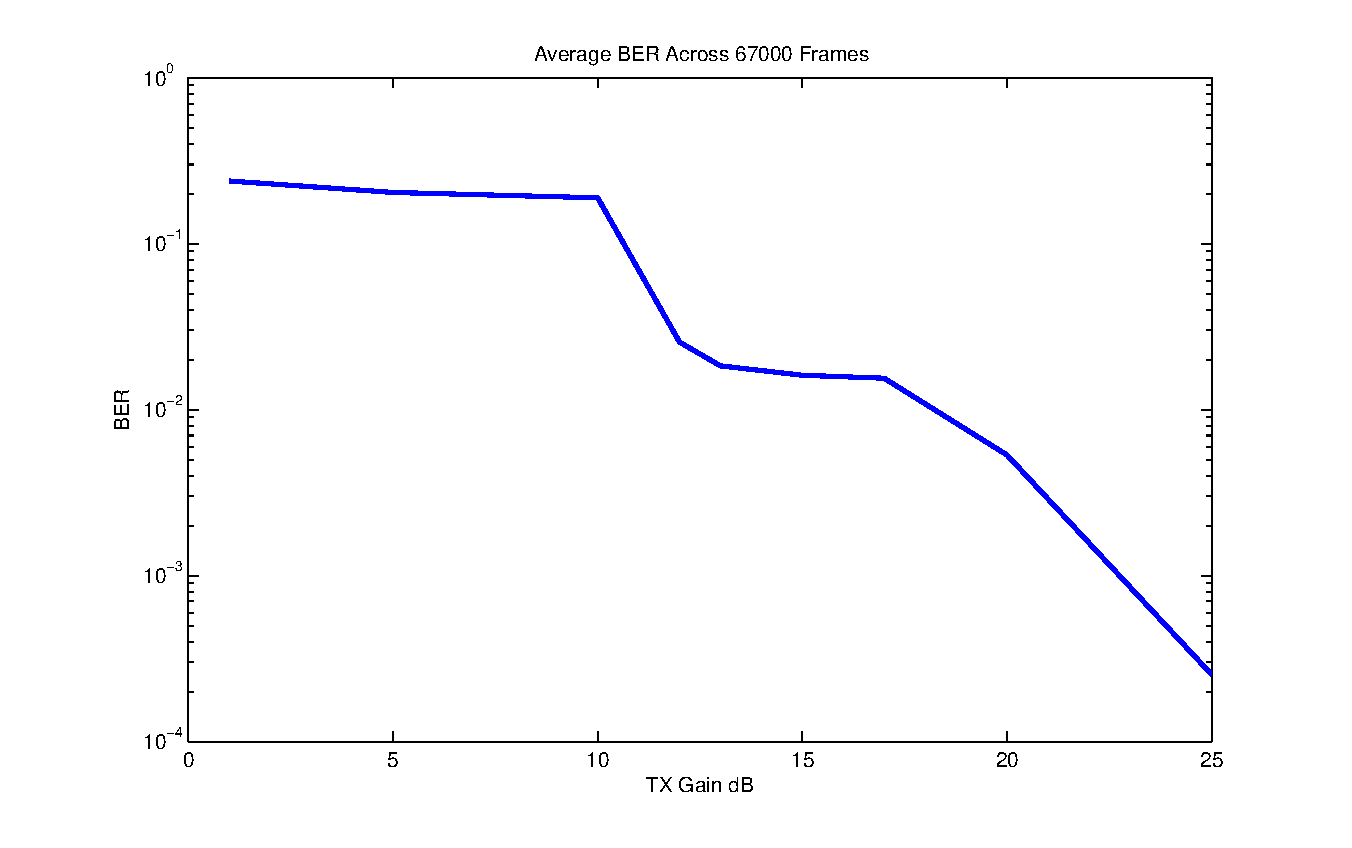
\includegraphics{ssep_snr_tests.eps}
\end{figure}

Since only antennas are provided by the AntSS block, MRC will suffer.  Higher performance will be provided by more input signals, but that would increase the complexity of the system significantly.  More input signals could be a future ally for BLISS system for future research.  For the current system architecture the results are acceptable given the limitations and variability in the hardware itself.\\
ADD MORE\\

\section{Antenna Subset Selection}

Since Anteena Subset Selection was done by outside contractors, no analysis will be provided by this thesis.  

\section{Summary}


